% Geometric Fields Mechanics: Sigma Construction
% Author: Antonio miti

\documentclass[border=10pt]{standalone}
\usepackage{tikz}


\usetikzlibrary{arrows,positioning}
\tikzset{%
  % Specifications for style of arrows:
   projection/.style={
           ->,
           shorten <=1pt,
           shorten >=1pt,},
   lagmap/.style={
           projection,
           red},
   hammap/.style={
           projection,
           blue},
   inclusion/.style={
   		   left hook->,
           shorten <=1pt,
           shorten >=1pt,},                            
  % Specifications for style of nodes:
   base/.style = {rectangle, rounded corners, draw=black,
                  minimum width=2.5cm, minimum height=1cm,
                  text centered, font=\sffamily},
   manifold/.style = {rectangle, rounded corners, draw=black,
                  minimum width=2.5cm, minimum height=2.5cm,
                  text centered, font=\sffamily},
   tangent/.style = {circle, rounded corners, draw=black,
                  minimum width=3cm, minimum height=1cm,
                  text centered, font=\sffamily},
      tangent/.style = {circle, rounded corners, draw=black,
                  minimum width=3cm, minimum height=1cm,
                  text centered, font=\sffamily},               
   verticalsmall/.style = {rectangle, rounded corners, draw=black,
                  minimum width=1cm, minimum height=1cm,
                  text centered, font=\sffamily},
   verticalbig/.style = {rectangle, rounded corners, draw=black,
                  minimum width=1.75cm, minimum height=1.75cm,
                  text centered, font=\sffamily},                              
   hamiltonian/.style = {base, fill=blue!20},
   lagrangian/.style = {base, fill=red!20},
   process/.style = {base, minimum width=1cm,
                     font=\ttfamily},
}

\begin{document}    

% Drawing part, node distance is 1.5 cm and every node
% is prefilled with white background

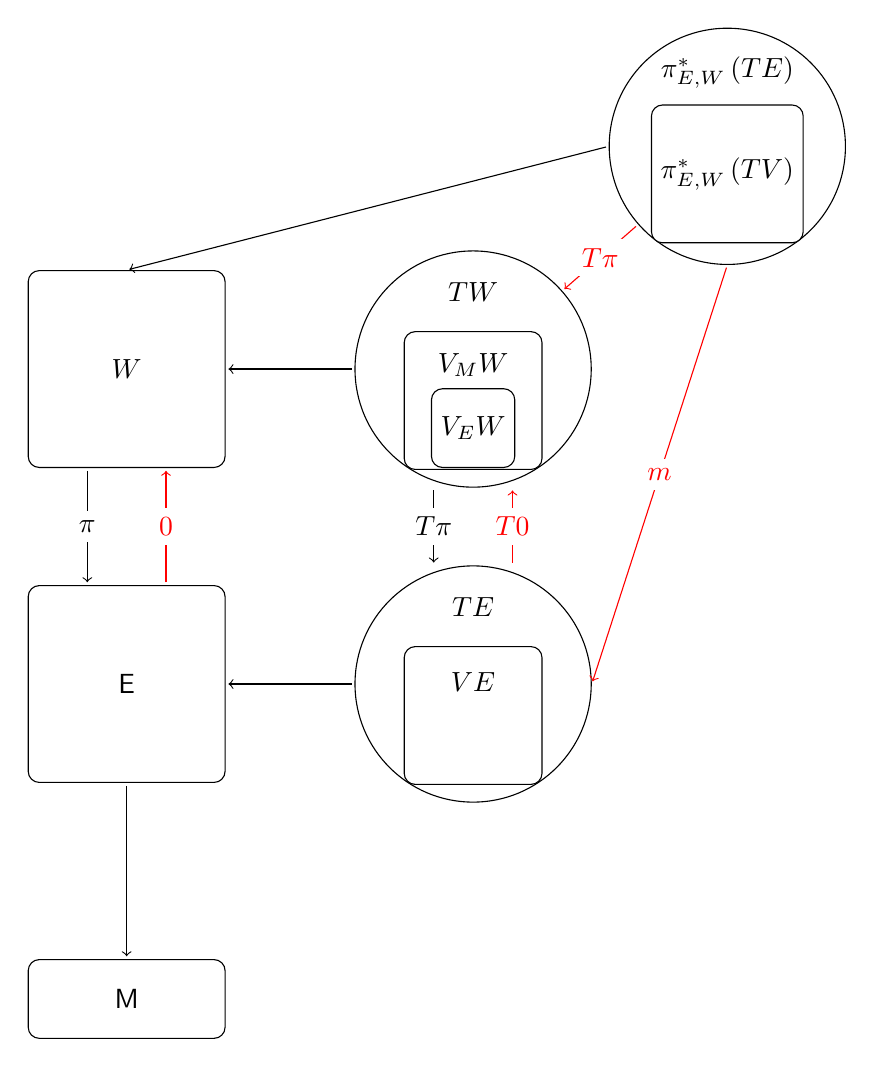
\begin{tikzpicture}[node distance=4cm,
    every node/.style={fill=white, font=\sffamily}, align=center]

  % Specification of nodes (position, etc.)
  \node (M_block)	[base]	{M};
  \node (E_block)	[manifold, above of= M_block]	{E};
  \node (W_block)	[manifold, above of= E_block]	{$W$};
  \node (TE_block)	[tangent, right of= E_block, , xshift=0.4cm , label={[label distance=-0.775cm]90:$TE$}]	{};
  \node (VE_block)	[verticalbig, right of= E_block,xshift=0.4cm, yshift=-0.40cm, label={[label distance=-0.7cm]90:$VE$}]	{};

  \node (TW_block)	[tangent, right of= W_block, , xshift=0.4cm , label={[label distance=-0.775cm]90:$TW$}]	{};
  \node (VmW_block)	[verticalbig, right of= W_block, , xshift=0.4cm, yshift=-0.40cm, label={[label distance=-0.7cm]90:$V_M W$}]	{};
  \node (VeW_block)	[verticalsmall, right of= W_block, ,  xshift=0.4cm, yshift=-0.75cm]	{$V_EW$};

  \node (pbTW_block) [ tangent, above right of= TW_block, xshift=0.4cm , label={[label distance=-0.9cm]90:$\pi_{E,W}^\ast\left( TE\right)$}]	{};
  \node (pbVmW_block)	[verticalbig, above right of= TW_block , xshift=0.4cm, yshift=-0.35cm]	{$\pi_{E,W}^\ast\left( TV\right)$};


  % Bundle Projections 
	\draw[projection]	(E_block) -- (M_block);
	\draw[projection]	([xshift=-0.5cm]W_block.south) -- node {$\pi$} ([xshift=-0.5cm]E_block.north);
	\draw[projection]	(TE_block) -- (E_block);
	\draw[projection]	(TW_block) -- (W_block);
	\draw[projection]	(pbTW_block.west) -- (W_block.north);
	
	\draw[lagmap]	(pbTW_block.south) -- node {$m$}	(TE_block.east);   
	\draw[projection]	([xshift=-0.5cm]TW_block.south) -- node {$T \pi$}	([xshift=-0.5cm]TE_block.north); 
	\draw[lagmap]	([xshift=+0.5cm] E_block.north) -- node {$0$}	([xshift=+0.5cm] W_block.south);    
	\draw[lagmap]	([xshift=+0.5cm] TE_block.north) -- node {$T 0$}	([xshift=+0.5cm] TW_block.south);   	
	\draw[lagmap]	(pbTW_block) -- node {$T \pi$}	(TW_block);   

  \end{tikzpicture}
\end{document}